\documentclass[11pt, a4paper]{report}
\usepackage{setspace}
%\usepackage{subfigure}

% Page styling
%\pagestyle{plain}
\usepackage{amssymb,graphicx,color}
\usepackage{amsfonts}
\usepackage{extsizes}
\usepackage{latexsym}
\usepackage[a4paper,margin=3cm]{geometry}
\usepackage{changepage}
\usepackage{mathptmx}

% Fancy style

% Tables
\usepackage{multirow, multicol}
\setlength{\columnsep}{1cm}

% Custom theorems
\usepackage[font=small, labelfont=bf]{caption}
\usepackage[protrusion=true, expansion=true]{microtype}
\usepackage{sectsty}
\usepackage{url, lipsum}
\usepackage{amsthm}

\usepackage{hyperref}

\theoremstyle{definition}
\newtheorem{theorem}{THEOREM}
\newtheorem{lemma}[theorem]{LEMMA}
\newtheorem{corollary}[theorem]{COROLLARY}
\newtheorem{proposition}[theorem]{PROPOSITION}
\newtheorem{remark}[theorem]{REMARK}
\newtheorem{definition}[theorem]{DEFINITION}
\newtheorem{fact}[theorem]{FACT}
\newtheorem{example}[theorem]{EXAMPLE}
\newtheorem{property}[theorem]{PROPERTY}

% Positioning figures
\usepackage{float}
\usepackage[demo]{graphicx}
\usepackage{subfig}

% Equations
\usepackage{amsmath}

% Code
\usepackage{fancyvrb}

% Spacing
\newcommand{\HRule}[1]{\rule{\linewidth}{#1}}
\setcounter{tocdepth}{5}
\setcounter{secnumdepth}{5}

% Helper packages - delete these before submission
\usepackage{xcolor}


%----------------------------------------------------------------------------------
% Title Page
%----------------------------------------------------------------------------------
\title{{\vspace{-2in}
\includegraphics[scale=0.4]{docs/Project Report/Media/ucl_logo.png}}\\
\vspace{2cm}
\begin{adjustwidth}{1cm}{1cm}
    \centering
    \Huge Robust Robotic Grasping Utilising Touch Sensing
\end{adjustwidth}}
\\
\date{Submission date: \today}
\author{Koo Ho Tin Justin\thanks{
{\bf Disclaimer:}
This report is submitted as part requirement for the BSc degree in Computer Science at UCL. It is
substantially the result of my own work except where explicitly indicated in the text.
\emph{Either:} The report may be freely copied and distributed provided the source is explicitly acknowledged
\newline  %% \\ messes it up
\emph{Or:}\newline
The report will be distributed to the internal and external examiners, but thereafter may not be copied or distributed except with permission from the author.}
\\ \\
BSc Computer Science\\ \\
Supervisors: Prof. Marc Deisenroth, Dr. Yasemin Bekiroglu}



\begin{document}
\onehalfspacing
\maketitle


%----------------------------------------------------------------------------------
% Abstract
%----------------------------------------------------------------------------------
\begin{abstract}
Robotic grasp synthesis has been studied extensively as robotic grasping skills have a significant impact on the success of subsequent manipulation tasks. Various approaches have been proposed for robotic grasp planning, with different assumptions regarding the available information about the type of objects in question (known, unknown, familiar). These approaches range from heuristic rules, designing simplifying hand models, to completely end-to-end systems inferring grasp parameters from raw data.\\

However, the majority of these approaches do not address robustness in grasping, which refers to the ability of a robot to perform a grasping task consistently and accurately even in the case of unexpected disturbances or large degree of errors in perception. There are several fundamental problems that need to be addressed for achieving better robustness in grasping tasks. These include mainly dealing with uncertainties in sensing, actuation and the perceptual data.\\

In this project, we study how to build a robust learning framework that can be employed to construct robust grasp configurations using multi-modal data, e.g. tactile, and visual. The project addresses the following main issues with the robotic grasping systems: a) balancing the trade-off between data representation and data dimensionality; b) analyzing the modelling effects of different modalities, e.g. tactile and visual, and features to capture the underlying characteristics of the overall grasping process; c) a correction policy that relies on assessing grasp success before further manipulation using perceptual data, to choose the right grasping configuration.
\end{abstract}


%----------------------------------------------------------------------------------
% Acknowledgements
%----------------------------------------------------------------------------------
\renewcommand\abstractname{Acknowledgments}
\begin{abstract}
    
\end{abstract}


%----------------------------------------------------------------------------------
% Contents
%----------------------------------------------------------------------------------
\tableofcontents
\setcounter{page}{1}


%----------------------------------------------------------------------------------
% Chapter 1: Introduction
%----------------------------------------------------------------------------------
\chapter{Introduction}
\label{chap:1}

\section{Outline of Problem}
\label{sec:1.1}
The field of robotic grasping has seen remarkable advancements in recent years, driven by the convergence of machine learning, computer vision, and robotics. This technology has the potential to be utilised in manufacturing, warehouse automation and household robotics. However, the development of robust and efficient grasping systems presents several challenges.\\

Robustness in a robotic grasping system refers to its versatility of accurately recognising and grasping objects with varying geometric features (width, depth, curvature, etc). Robustness is increasingly becoming a vital factor in the study of grasp stability and quality. However, facilitating robustness makes it practically difficult to design a single gripper that can effectively grasp all objects. As a result, researchers and engineers have developed dedicated grippers tailored to specific grasping tasks or types of objects.\\

The project first analyses various literature concerned with learning frameworks to robotic grasping that involves different combinations of sensory (tactile and visual) data. These frameworks mainly adapt either a learning-based approach to formulate a regrasping policy, or tactile exploration to maximise grasp quality and improve object shape representation.\\

Backed with survey findings, a simple Pybullet simulation is developed to collect tactile and visual data. This data is essential for training a logistic regression classifier to tackle a binary classification problem for good and bad labelled grasps. The classifier serves as the baseline approach for the project and a means to discover the best data representation for the data in question.\\

Finally, the project will propose a learning framework that infers hand poses for good grasps using a generative model with Gaussian processes. The framework is also tested on a real setup of the robot and the performances will be displayed and analysed in depth.


\section{Project Aims and Objectives}
\label{sec:1.2}

\subsection{Project aims}
\label{sec:1.2.1}
The aim of this project is for the development and testing of a robust robotic system that can learn to pick up an object with simple geometry using a two-finger hand. The project will take a learning-based approach to grasping through, for example, Bayesian optimization \cite{nogueria, frazier}. The learning-based approach should be compared with a baseline approach from the related literature (e.g. \cite{nogueria, danielczuk, breyer}) for evaluation. 

\subsection{Objectives}
\label{sec:1.2.2}
The project aim is divided into several objectives that are expected to be completed throughout the academic year. 
\begin{enumerate}
    \item Set up a simulation environment, e.g. PyBullet or NVIDIA Isaac. 
    \item Create a data collection pipeline for sensory data (e.g. visual and force/torque readings) via the simulator.
    \item Apply basic simulation functionalities: position control and vision sensing on the robot.
    \item Implement and test baseline (e.g. \cite{breyer}, and a basic approach such as executing predefined grasps per object model given object pose).
    \item Build the learning framework:
    \begin{enumerate}
        \item Learning grasps based on Bayesian Optimization, from a chosen scene representations such as signed distance function 
        \item Picking with two fingers given object model (primitive shapes such as box, sphere, cylinder) and pose, all learned by trial and error
    \end{enumerate}
\end{enumerate}

\newpage
\section{Project Approach}
\label{sec:1.3}
We approached the project in four stages:
\begin{enumerate}
    \item Carry out background reading on robotic grasping, including policy learning, regression methods and grasp inference
    \item Implement of a simple Pybullet environment consisting of a robot arm, gripper and DIGIT tactile sensors
    \item Develop a data collection pipeline to gather tactile and visual data for rigid bodies in the simulation
    \item Implement and test a baseline approach using the simulation
    \item Implement and test the proposed learning-based approach using the simulation.
\end{enumerate}
Any technologies and tools required for the project will also be stated and justified in the corresponding sections.


\section{Report Structure}
\label{sec:1.4}
Chapter 2 covers the background and literature review for the project, including important terms and definitions, core packages for the project as well as the analysis of several related literature concerning the data representation of tactile, sensory and temporal data, robotic regrasping approaches and tactile exploration.\\

Chapter 3 documents the development of the Pybullet simulation for the project and the experimentation and analysis of physical DIGIT sensors.\\

Chapter 4 documents the development and testing of the baseline approach logistic regression classifier). It incorporates findings from Chapter 2 to discover the best data representation (raw, PCA, CNN) and the type of data to include (tactile only, visual only, both).\\

Chapter 5 documents the development and implementation of the proposed approach using a Gaussian process generative model that attempts to infer good grasp configurations from random hand poses.\\

Chapter 6 summarises the results and performances of the project, as well as making suggestions for future work and improvement based on these findings.


%----------------------------------------------------------------------------------
% Section 2: Literature Review
% Focuses on important terms used throughout the report & academic papers read in-depth
%----------------------------------------------------------------------------------
\chapter{Background and Literature Review}
\label{chap:2}

\section{Robotic Grasping}
\label{sec:2.1}
Robotic grasping refers to the ability of a robot to pick up and manipulate objects using its mechanical grippers or other end effectors. It requires precise coordination between the visual perception of the environment and efficient grasp planning, as well as robustness in terms of the object type, which is the main focus of this project.\\

There are several challenges in robotic grasping, such as object recognition, pose estimation, and grasp planning. To grasp an object, a robot needs to detect the object's location (through, for example, a wrist camera), orientation, and size accurately, estimate the best grasp point and orientation, and then execute the grasp with appropriate force and control to ensure a secure hold. The grasping process can be performed using various types of end effectors, including grippers, suction cups, or specialized tools designed for specific tasks. In this project, we will use a pair of DIGIT tactile sensors mounted onto each finger of the gripper to collect sensory readings.


\section{Pybullet}
\label{sec:2.2}
Pybullet \cite{pybullet} is a physics engine and simulator designed to be used in robotics, machine learning and computer graphics. It is a Python wrapper for the Bullet Physics Library, which is an open-source physics engine that can simulate rigid body dynamics, soft body dynamics, and fluids.


These components are collectively controlled by the robot's control system, which is responsible for controlling the movement of the arm, processing sensor data, and coordinating the actions of every component. The control system may be a simple physical microcontroller, but in the context of this project, we will use the Pybullet \cite{pybullet} package to achieve our robot manipulation functions.

\section{Related Literature}
\label{sec:2.3}


\subsection{More Than a Feeling: Learning to Grasp and Regrasp using Vision and Touch (Calandra et al)\cite{calandra}}
\label{sec:2.3.1}
Humans rely on rich tactile feedback to grasp objects, however, most of the recent robotic grasping studies only focus on visual input. The authors propose an end-to-end action-conditional model (a multimodal CNN) to learn regrasping policies from visual-tactile data, by predicting outcome of a candidate grasp adjustment, then executing a grasp by iteratively selecting the most promising actions\cite{calandra}.


\subsection{Generalizing Regrasping with Supervised Policy Learning (Hausman et al)\cite{hausman}}
\label{sec:2.3.2}


\subsection{Simultaneous Tactile Exploration and Grasp Refinement for Unknown Objects (Farias et al)\cite{farias}}
\label{sec:2.3.3}


\section{Conclusion on Literature Review}
\label{sec:2.4}


%----------------------------------------------------------------------------------
% Section 3: Developing a Pybullet simulation
% Describes the detailed process of developing the simulation for the project
%----------------------------------------------------------------------------------
\chapter{Experimentation and Development of Pybullet Simulation}
\label{chap:3}

\section{Implementation of basic functionalities}
Arm control, grasp control, position control, gripper control, get 6d pose, reset

\section{Parameters}
yaml parameters, loading parameters


%----------------------------------------------------------------------------------
% Section 4: Designing a Baseline Model and Deciding on Feature Representation of Tactile and Visual Data
%----------------------------------------------------------------------------------
\chapter{Baseline and Feature Representation Analysis}
\label{chap:4}
Given different combinations of multi-modal data (tactile and visual) collected from grasping an object, we would like to a) determine whether the outcome (successful or unsuccessful) of the grasp is ascertainable based on this data; and b) determine the best feature representation for said data.

\section{Multi-modal Data Collection}
\label{sec:4.1}
In this experiment, we collect tactile and visual data on a smooth rectangular block by executing randomly-generated end effector poses.

\subsection{Generating Random Grasps}
\label{sec:4.1.1}
Using our Pybullet simulation, we manually manipulate the end effector to varying positions in the proximity of the block, and record three different end effector poses ($i=0,1,2$) to guarantee some variation in the orientation and position of the grasps. Each end effector pose $S_i$ is a 6-tuple consisting of 3 Cartesian coordinates representing the spatial position of the end effector relative to the robot, and 3 Euler angles representing the orientation of the end effector:
\begin{equation}
    S_i=(x,y,z,\alpha,\beta,\gamma)
\end{equation}
We treat each manually-selected pose independently as a seed grasp configuration, and generate a pre-determined number $N$ of random poses $X_n$ from the seed by adding a small amount of Gaussian noise $K_n$ ($\mu=0$ and $\sigma=0.01$) to each dimension of the seed pose. Mathematically, for every $S_i$, the randomly generated grasps are denoted as:
\begin{equation}
    X_n=S_i+K_n
\end{equation}
where $K\sim N(0,0.01)$. To prevent collision between the gripper and the object when initializing the end effector pose, we add some padding to the z-dimension, denoted as $p_z$.

\subsection{Data Collection}
\label{sec:4.1.2}
We execute each randomly-generated pose $X_n$ by commanding the robot to perform a simple pick-and-place task. First, it needs to move the end effector to the desired position $X_n$, with a padding distance of $p_z$ to avoid colliding with the object. Then, it lowers the end effector vertically by an offset of $p_z$ to reach the target object. Once the end effector is in position, the robot closes the gripper to perform the grasp on the object. To ensure grasp stability, the robot measures the number of contact points between the two fingers and the object. If the gripper is in stable contact, the robot records depth and color tactile data using the DIGIT tactile sensors.\\

Before lifting the object, the robot performs a sanity check on the recorded tactile data. This is extremely important as it prevents adding meaningless data (Fig. \ref{fig:1}) to the training dataset.
\begin{figure}[H]%
    \centering
    \subfloat[\centering Invalid tactile data]{{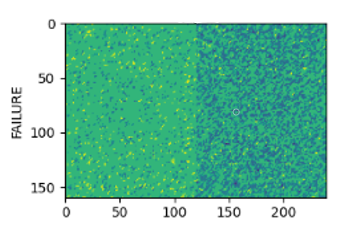
\includegraphics[width=7cm]{docs/Project Report/Media/4_1_2_failed_tactile_data.png} }}%
    \qquad
    \subfloat[\centering Valid tactile data]{{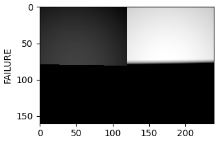
\includegraphics[width=6.7cm]{docs/Project Report/Media/4_1_2_valid_tactile_data.png} }}%
    \caption{Sanity check for tactile data}%
    \label{fig:1}%
\end{figure}

Once the robot verifies that the object is stably held, it lifts the object vertically by an offset of $p_z$ to return to $X_n$. Finally, the robot determines the outcome of the grasp by detecting the change in the object's z-position.

\section{Data Sampling and Pre-processing}
\label{sec:4.2}
Data was processed in 3 ways: raw, PCA with 3 main components, Convnet

\section{Visualising the Dataset}
Add skeleton hand plot, and some subplots of color and depth images

\section{Baseline Model Training}

\section{Evaluation of Baseline Model Results}

\section{Conclusion}
\subsection{Feature Representation}
Select the most promising representation and use it for actual generative model in Sec 4.

\subsection{Analysis of Results}

%----------------------------------------------------------------------------------
% Section 5: Actual Model
%----------------------------------------------------------------------------------
\chapter{Actual Model}
\label{chap:5}

\section{Multilayer Perceptron}
2 layers

\section{Data representation}
CNN dimension-reduced data

\section{Training}

\section{Validation}

\section{Interesting experiments}
\begin{itemize}
    \item Train with data of 2 blocks, test with data of 1 block
    \item Train with data of multiple types of objects (e.g. block + cylinder)
\end{itemize}



%----------------------------------------------------------------------------------
% Section 5: Future Work
%----------------------------------------------------------------------------------
\chapter{Future Work}
\label{chap:6}
Since Pybullet is no longer being maintained, consider to move to mujico



%----------------------------------------------------------------------------------
% Appendix section
%----------------------------------------------------------------------------------
\appendix


\begin{thebibliography}{9}
% Academic papers
\bibitem{haarnoja}
    Haarnoja, T., Zhou, A., Abbeel, P. & Levine, S..
    \textit{Soft Actor-CriticL Off-Policy Maximum Entroy Deep Reinforcement Learning with a Stochastic Actor, \href{https://arxiv.org/abs/1801.01290}{https://arxiv.org/abs/1801.01290}},
    ICML,
    2018 roboti

\bibitem{nogueria}
    Nogueria et al,
    \textit{Unscented Bayesian Optimization for Safe Robot Grasping},
    IROS,
    2016

\bibitem{danielczuk}
    Danielczuk et al,
    \textit{Exploratory Grasping: Asymptotically Optimal Algorithms for Grasping Challenging Polyhedral Objects},
    2020

\bibitem{bekiroglu}
    Bekiroglu et al,
    \textit{Assessing Grasp Stability from Haptic Data},
    IEEE TRO,
    2011

\bibitem{frazier}
    Frazier,
    \textit{A Tutorial on Bayesian Optimization},
    2018

\bibitem{breyer}
    Breyer,
    \textit{\href{https://github.com/ethz-asl/vgn}{https://github.com/ethz-asl/vgn}}
    CORL,
    2020

% Academic papers for survey
\bibitem{calandra}
    Calandra et al,
    \textit{More Than a Feeling: Learning to Grasp and Regrasp using Vision and Touch},
    2018

\bibitem{hausman}
    Hausman et al,
    \textit{Generalizing Regrasping with Supervised Policy Learning},
    2017

\bibitem{farias}
    Farias et al,
    \textit{Simultaneous Tactile Exploration and Grasp Refinement for Unknown Objects},
    2021

% References for technologies used
\bibitem{digit}
    \href{https://digit.ml/}{DIGIT tactile sensors, 2020 @ Facebook}

\bibitem{pybullet}
    \href{https://pybullet.org/wordpress/}{Pybullet}

@article{Wang2022TACTO,
  author   = {Wang, Shaoxiong and Lambeta, Mike and Chou, Po-Wei and Calandra, Roberto},
  title    = {{TACTO}: A Fast, Flexible, and Open-source Simulator for High-resolution Vision-based Tactile Sensors},
  journal  = {IEEE Robotics and Automation Letters (RA-L)},
  year     = {2022},
  volume   = {7},
  number   = {2},
  pages    = {3930--3937},
  issn     = {2377-3766},
  doi      = {10.1109/LRA.2022.3146945},
  url      = {https://arxiv.org/abs/2012.08456},
}

\bibitem{franka}
    \href{https://www.franka.de}{Franka Emika}

\bibitem{robotiq}
    \href{https://robotiq.com/products/2f85-140-adaptive-robot-gripper}{Robotiq}

\end{thebibliography}

\chapter{Other appendices, e.g., code listing}
Put your appendix sections here

\end{document}